\documentclass[conference]{IEEEtran}
\IEEEoverridecommandlockouts
\usepackage{cite}
\usepackage{amsmath,amssymb}
\usepackage{graphicx}
\usepackage{booktabs}
\usepackage{xcolor}
\usepackage{url}
\usepackage[hidelinks]{hyperref}
\graphicspath{{../docs/figures/}}
\makeatletter
\newcommand{\linebreakand}{%
  \end{@IEEEauthorhalign}\hfill\mbox{}\par
  \mbox{}\hfill\begin{@IEEEauthorhalign}}
\makeatother

\begin{document}

\title{Instruction and Data Memory Hierarchy:\\
A Harvard-Style Memory Organisation in Verilog\\
and its Comparison with a Shared (Von Neumann) Memory\\
{\large Phase I Report -- Modern Computer Architecture, Project 9}}

\author{
\IEEEauthorblockN{Aaryan Yadav}
\IEEEauthorblockA{2401010011}
\and
\IEEEauthorblockN{Shashwat Sinha}
\IEEEauthorblockA{2401010438}
\and
\IEEEauthorblockN{Shivam Mishra}
\IEEEauthorblockA{2401010442}
\and
\IEEEauthorblockN{Himank Kaushik}
\IEEEauthorblockA{2401010187}
\and
\IEEEauthorblockN{Satyam Kumar}
\IEEEauthorblockA{2401010429}
\linebreakand
\IEEEauthorblockA{\textit{B.Tech CSE (AI), Rishihood University, Sonipat, Haryana, India}}
}

\maketitle

% ---------------------------------------------------------------------------
\begin{abstract}
A processor needs memory for two different things: the instructions it runs
and the data those instructions work on. In a Von Neumann (shared-memory)
machine both travel over one bus, so a load or store has to wait while the
next instruction is fetched---a structural hazard often called the
\emph{Von Neumann bottleneck}. A Harvard organisation gives instructions and
data their own memories and buses, so both accesses can happen in the same
clock cycle. This project implements, in synthesisable Verilog, a simplified
Harvard memory hierarchy---program counter, 4\,KB instruction memory, 4\,KB
data memory, an address decoder, a read/write control unit and memory-mapped
I/O---driven by a single-cycle RV32I-subset processor. To make the comparison
fair, the \emph{same} processor RTL is also connected to a single-ported
unified memory through a two-state arbiter, forming a Von Neumann baseline.
Four test programs (array sum, vector add, bubble sort and Fibonacci) are run
on both systems with a self-checking testbench that compares every data-memory
word with a Python golden model. All eight runs pass. The Harvard design
completes every program at CPI\,=\,1.00, while the shared-memory baseline
reaches CPI of 1.02--1.31, so the Harvard organisation is up to
$1.31\times$ faster, with the gain growing linearly with the fraction of
load/store instructions. This Phase I report covers the literature, the
proposed architecture, the working prototype and the team's contributions.
\end{abstract}

\begin{IEEEkeywords}
Harvard architecture, Von Neumann architecture, memory hierarchy,
instruction memory, data memory, address decoding, RISC-V, Verilog, structural hazard
\end{IEEEkeywords}

% ---------------------------------------------------------------------------
\section{Introduction}
Every instruction a processor executes has to be \emph{fetched} from memory,
and roughly a quarter to a third of typical instructions also \emph{read or
write data} in memory. How the memory system is organised therefore decides
whether these two kinds of access can overlap or must take turns.

The objective of this project, as defined in the course project list
\cite{mca_projects}, is to ``implement a simplified Harvard-style memory
organisation with separate instruction and data paths and analyse its
behaviour''. Concretely we (i) build independent instruction and data paths
in Verilog, (ii) connect them to a simple processor, (iii) execute programs
that contain both instruction fetches and data accesses, (iv) measure how
often both paths are used in the same cycle, and (v) compare against a
shared-memory organisation built from the same processor.

% ---------------------------------------------------------------------------
\section{Literature Review}

\subsection{Origins of the two organisations}
The stored-program concept described by von Neumann in the EDVAC report
\cite{vonneumann1945} keeps instructions and data in one memory. Its strength
is flexibility: programs are just data, so they can be loaded, modified or
generated at run time, and a single memory is cheaper to build. The Harvard
Mark~I \cite{aiken1946}, by contrast, read instructions from punched paper
tape and kept data in separate counters---the origin of the term
``Harvard architecture'' for machines with physically separate instruction
and data storage.

\subsection{The Von Neumann bottleneck and the memory wall}
Backus \cite{backus1978} named the single processor--memory channel the
``von Neumann bottleneck'': all instructions and all data must squeeze
through it one word at a time. As processor speed outgrew DRAM speed, Wulf
and McKee \cite{wulf1995} showed that average memory access time would come
to dominate performance (the ``memory wall''). Both arguments motivate
giving the processor more memory bandwidth, and the cheapest way to double
bandwidth for a pipeline is to split instruction and data traffic.

\subsection{Split memories in modern processors}
Textbook RISC datapaths \cite{patterson2020,harris2021} use separate
instruction and data memories precisely so that a single-cycle or pipelined
core can fetch an instruction and perform a load/store in the same cycle;
with a single memory, the MEM stage of one instruction collides with the IF
stage of a later one and a stall is required \cite{hennessy2017}. Real
systems use a \emph{modified Harvard} design: split level-1 instruction and
data caches \cite{smith1982} backed by a unified level-2 cache and main
memory, so programs still see one address space. Microcontrollers such as the
ARM Cortex-M3 expose separate ICode, DCode and System buses for the same
reason \cite{arm_m3}. Conversely, minimal cores such as PicoRV32
\cite{picorv32} deliberately use one unified memory interface to save area,
accepting extra cycles per memory instruction---exactly the trade-off this
project measures.

\subsection{Gap addressed by this project}
Most course designs show the Harvard datapath only as part of a full CPU and
never quantify what the split buys. Our contribution is a \emph{controlled}
comparison: identical processor RTL, identical programs and identical address
map, with only the memory organisation changed, and hardware performance
counters that measure the overlap directly.

% ---------------------------------------------------------------------------
\section{Proposed Solution}

\subsection{Overview and address map}
The processor core (\texttt{cpu\_core.v}) is a single-cycle RV32I subset
\cite{riscv_isa} supporting ADD, SUB, AND, OR, XOR, SLT, SLL, SRL, their
immediate forms, LW, SW, BEQ, BNE, BLT, BGE, JAL, JALR and LUI. It is
deliberately \emph{memory-organisation agnostic}: it exposes an instruction
port (PC $\rightarrow$ instruction) and a data port (address, write data,
read/write strobes $\rightarrow$ read data). Both systems share the address
map in Table~\ref{tab:map}.

\begin{table}[h]
\caption{Common address map}
\label{tab:map}
\centering
\begin{tabular}{lll}
\toprule
Range & Device & Access \\
\midrule
\texttt{0x0000\_0000--0FFF} & Instruction memory (4\,KB) & fetch \\
\texttt{0x0000\_1000--1FFF} & Data memory (4\,KB) & load/store \\
\texttt{0x0000\_2000} & I/O OUT register & store \\
\texttt{0x0000\_2004} & I/O HALT register & store \\
\texttt{0x0000\_2008} & I/O cycle counter & load \\
other & -- & bus error \\
\bottomrule
\end{tabular}
\end{table}

\subsection{Harvard organisation (proposed design)}
Fig.~\ref{fig:harvard} shows the proposed system (\texttt{harvard\_top.v}).
\begin{itemize}
\item \textbf{Program Counter} (\texttt{pc.v}) holds the fetch address and
supports a stall input.
\item \textbf{Instruction Memory} (\texttt{imem.v}) is a 1024-word ROM loaded
from a hex file with asynchronous read, so fetch and execute fit in one cycle.
\item \textbf{Address Decoder} (\texttt{addr\_decoder.v}) turns the upper
address bits of a load/store into one-hot chip selects for data memory or
I/O, and flags a bus error for unmapped addresses (including any data access
to the instruction region, which is illegal in a strict Harvard machine).
\item \textbf{Read/Write Control} (\texttt{rw\_control.v}) routes the core's
read/write strobes only to the selected device and multiplexes that device's
read data back to the core.
\item \textbf{Data Memory} (\texttt{dmem.v}) is a 1024-word RAM with
synchronous write and asynchronous read.
\item \textbf{Memory-mapped I/O} (\texttt{io\_regs.v}) provides a debug output
port, a HALT register used to end simulation, and a cycle counter.
\item \textbf{Performance counters} (\texttt{perf\_counters.v}) count cycles,
retired instructions, fetches, data reads/writes, stall cycles and
\emph{parallel} cycles in which a fetch and a data access occur together.
\end{itemize}

\begin{figure}[t]
\centering
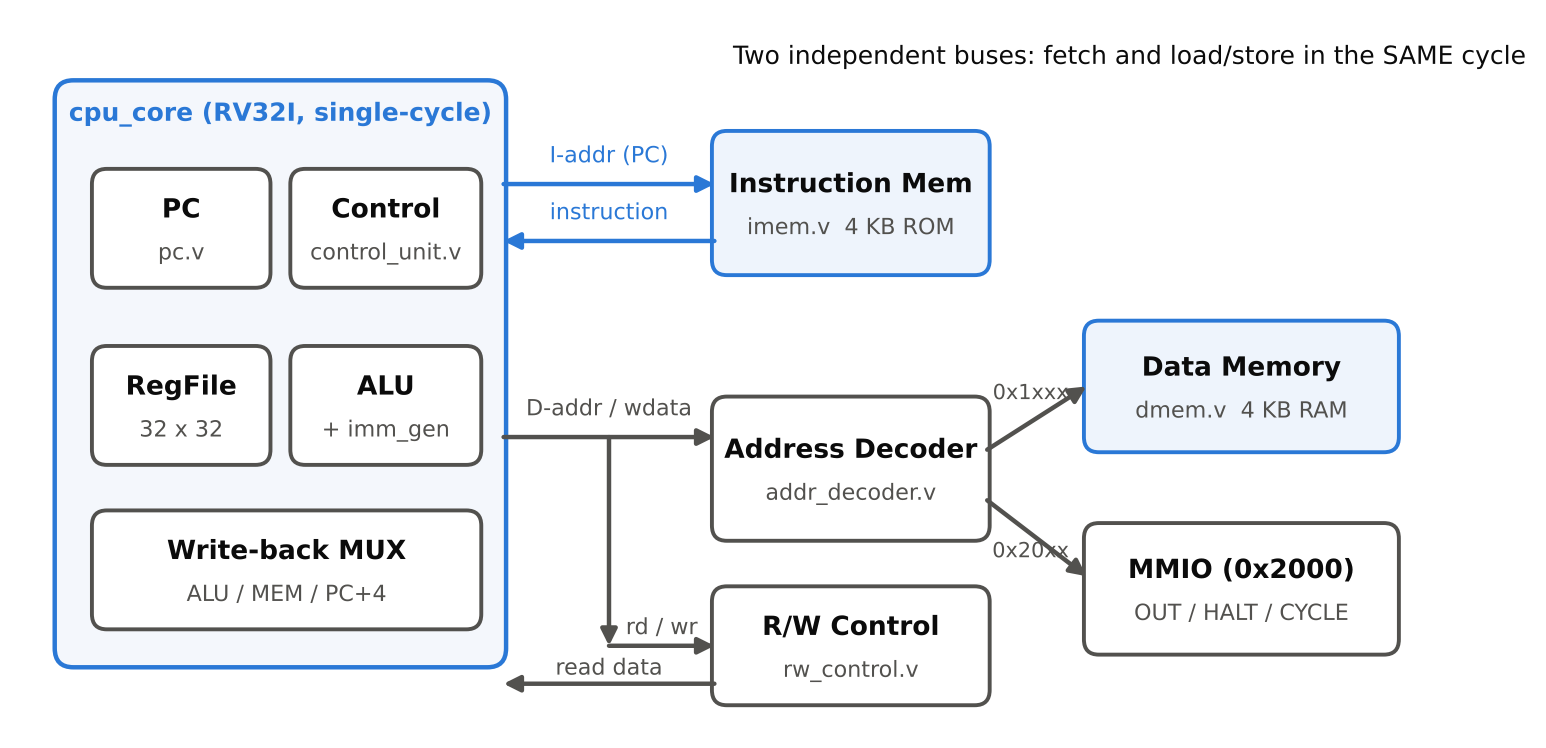
\includegraphics[width=\columnwidth]{block_harvard.png}
\caption{Proposed Harvard organisation: separate instruction and data buses.}
\label{fig:harvard}
\end{figure}

\subsection{Shared-memory baseline (Von Neumann)}
For comparison, \texttt{vonneumann\_top.v} connects the \emph{same}
\texttt{cpu\_core} to one single-ported 8\,KB memory holding both code and
data (Fig.~\ref{fig:vn}). A two-state arbiter resolves the structural hazard:
in \textsc{Fetch} the bus carries the PC; if the fetched instruction is a load
or store, it is latched into an instruction register, the core is stalled and
the arbiter moves to \textsc{Data}, where the bus carries the data address and
the latched instruction completes. Every load/store therefore costs two
cycles, giving the analytical model
\begin{equation}
\text{CPI}_{\text{H}} = 1, \qquad
\text{CPI}_{\text{VN}} = 1 + f_{\text{mem}}, \qquad
S = \frac{\text{CPI}_{\text{VN}}}{\text{CPI}_{\text{H}}} = 1 + f_{\text{mem}}
\label{eq:model}
\end{equation}
where $f_{\text{mem}}$ is the fraction of executed instructions that are
loads or stores.

\begin{figure}[t]
\centering
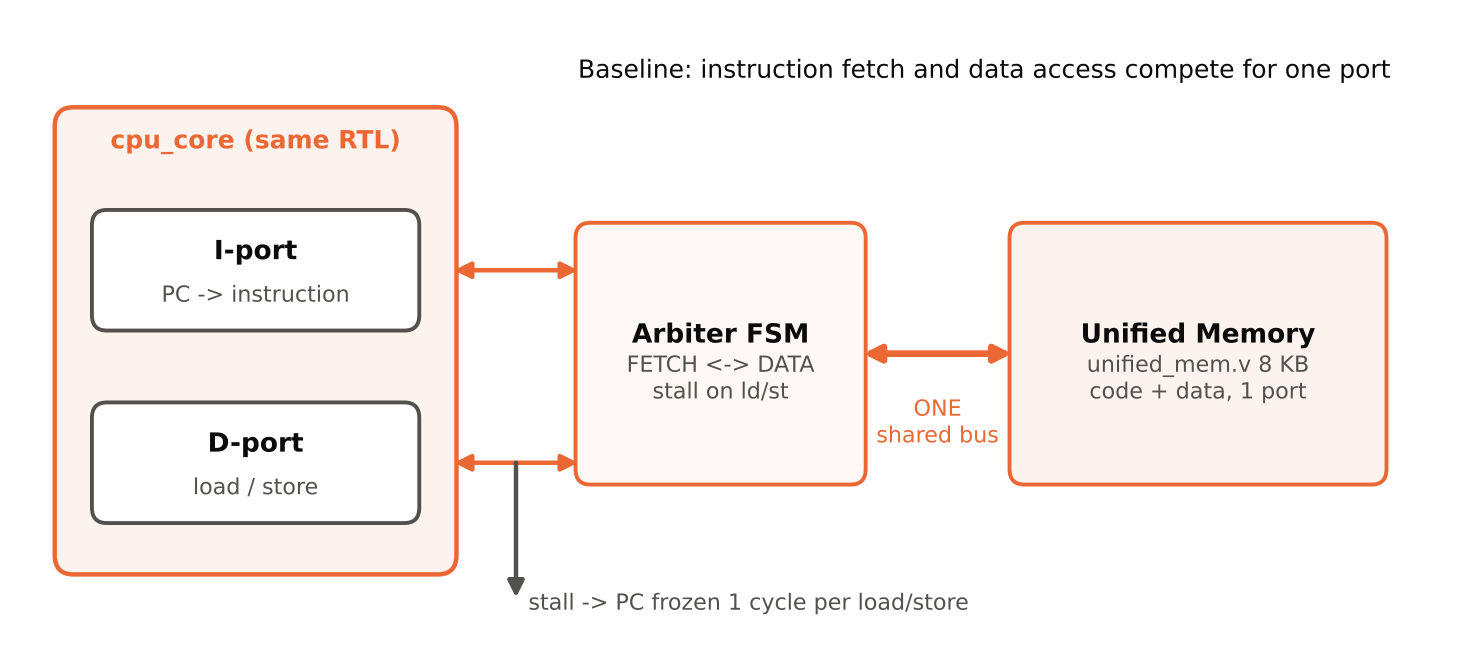
\includegraphics[width=\columnwidth]{block_vonneumann.png}
\caption{Baseline: unified single-port memory with fetch/data arbiter.}
\label{fig:vn}
\end{figure}

\subsection{Verification methodology}
A Python two-pass assembler and instruction-set simulator
(\texttt{sw/rv32\_asm.py}) produces, for each program, the instruction image,
the initial data image, the \emph{expected} final data-memory image and
predicted cycle counts from (\ref{eq:model}). The self-checking testbench
(\texttt{tb\_top.v}) runs either top level until the program writes the HALT
register, compares all 1024 data-memory words with the golden image, and
prints the hardware counters. A separate directed testbench checks the
address decoder and read/write control for nine cases (each region, region
boundaries, unmapped and aliased addresses, and no-request). Simulation uses
Icarus Verilog \cite{icarus}; waveforms are dumped as VCD.

\subsection{Phase I prototype status and preliminary results}
The prototype is complete and functionally verified: the decoder unit test
and all eight program/architecture runs pass, and every hardware cycle count
matches the analytical model exactly (Table~\ref{tab:res}).

\begin{table}[h]
\caption{Preliminary results (simulation, both designs)}
\label{tab:res}
\centering
\setlength{\tabcolsep}{4pt}
\begin{tabular}{lrrrrrr}
\toprule
Program & Instr. & $f_{\text{mem}}$ & H cyc. & VN cyc. & VN CPI & Speed-up \\
\midrule
fibonacci   & 128 & 1.6\%  & 128 & 130 & 1.02 & 1.02$\times$ \\
array\_sum  & 176 & 19.9\% & 176 & 211 & 1.20 & 1.20$\times$ \\
bubble\_sort& 633 & 31.1\% & 633 & 830 & 1.31 & 1.31$\times$ \\
vector\_add & 156 & 31.4\% & 156 & 205 & 1.31 & 1.31$\times$ \\
\bottomrule
\end{tabular}
\end{table}

Figs.~\ref{fig:waveh} and~\ref{fig:wavev} show the same 24-cycle window of
the \texttt{vector\_add} loop. In the Harvard design the instruction bus is
busy every cycle while loads and stores proceed alongside it; in the
baseline, every \texttt{lw}/\texttt{sw} takes the bus away from instruction
fetch for one cycle and the stall signal rises. The Harvard counters report
49 parallel cycles for \texttt{vector\_add}---exactly the number of stall
cycles the baseline suffers (Fig.~\ref{fig:cycles}).

\begin{figure*}[t]
\centering
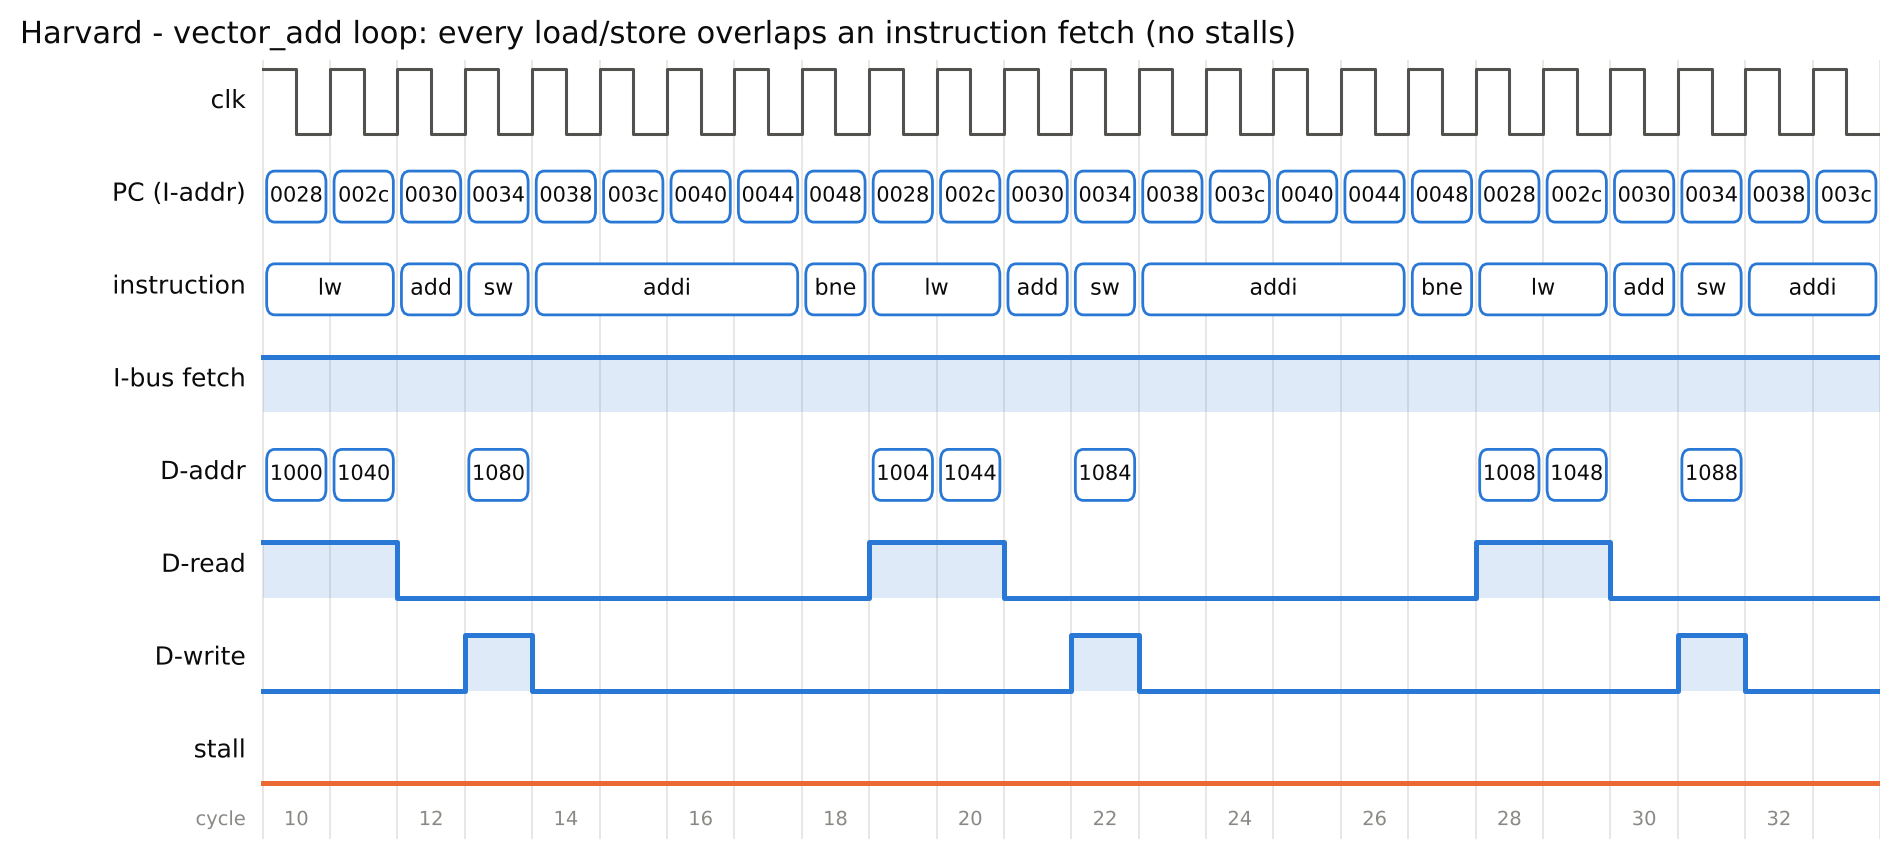
\includegraphics[width=0.85\textwidth]{wave_harvard.png}
\caption{Harvard waveform (\texttt{vector\_add}): fetch and load/store overlap; no stalls.}
\label{fig:waveh}
\end{figure*}

\begin{figure*}[t]
\centering
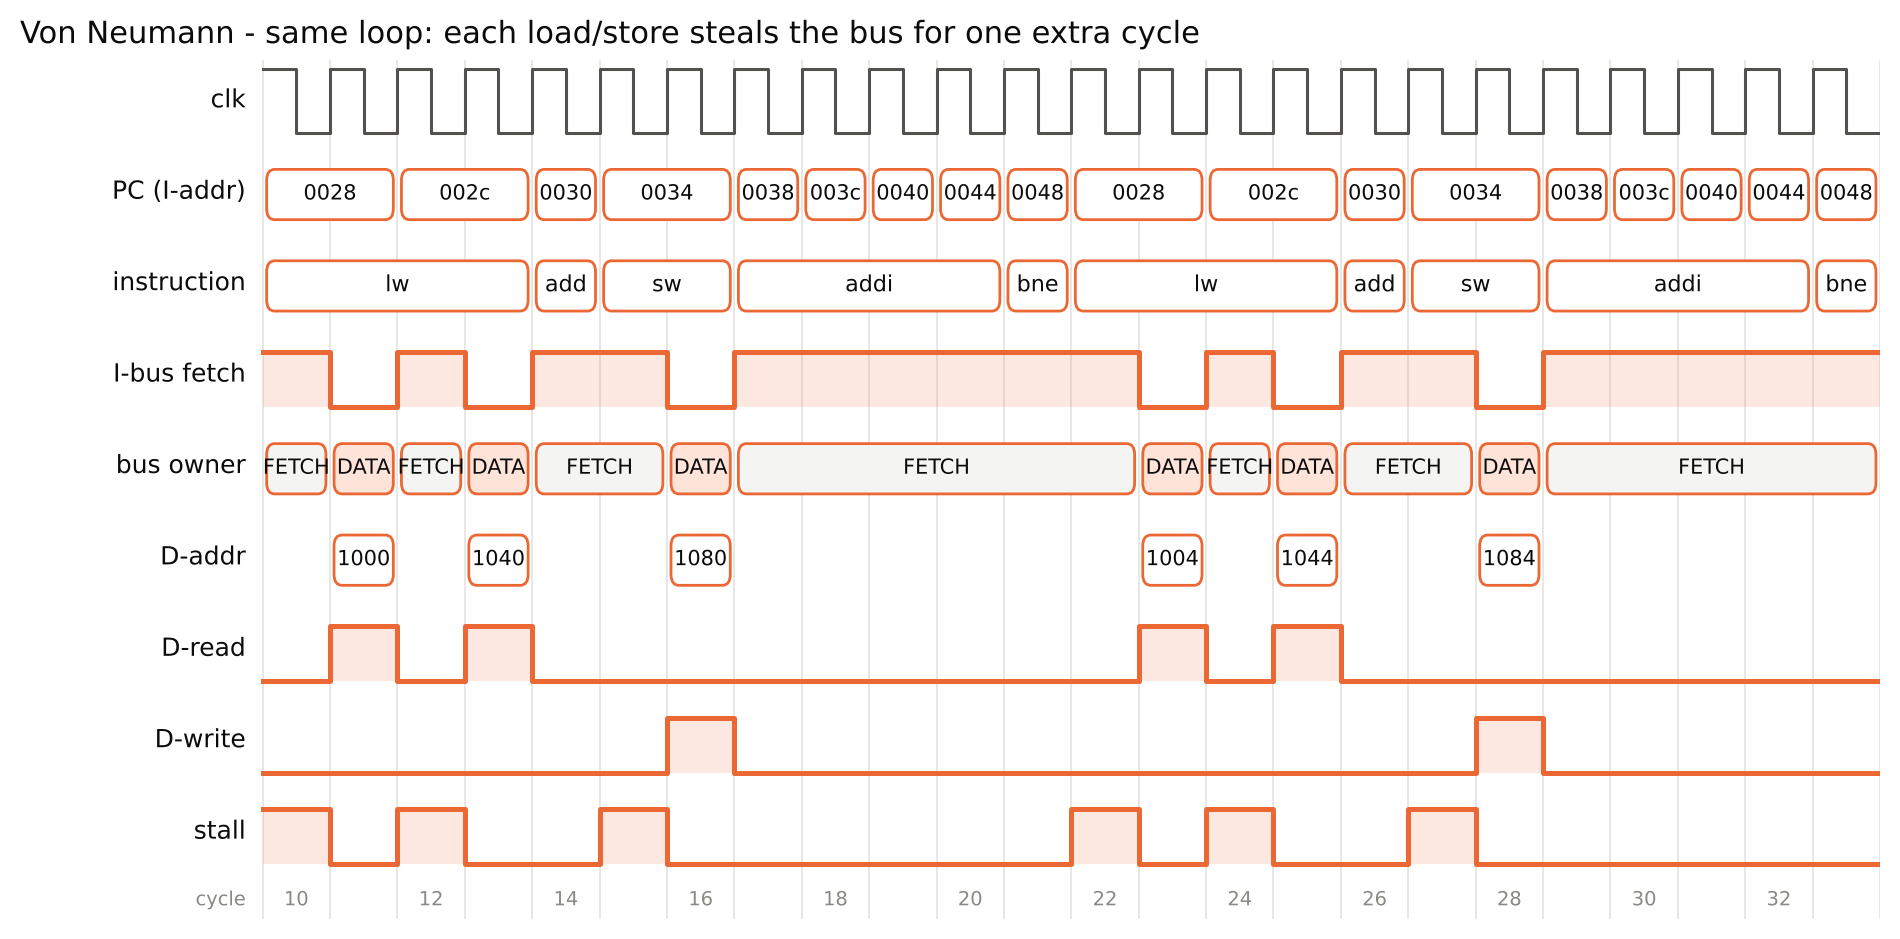
\includegraphics[width=0.85\textwidth]{wave_vonneumann.png}
\caption{Von Neumann waveform (\texttt{vector\_add}): each load/store adds a DATA cycle on the shared bus.}
\label{fig:wavev}
\end{figure*}

\begin{figure}[t]
\centering
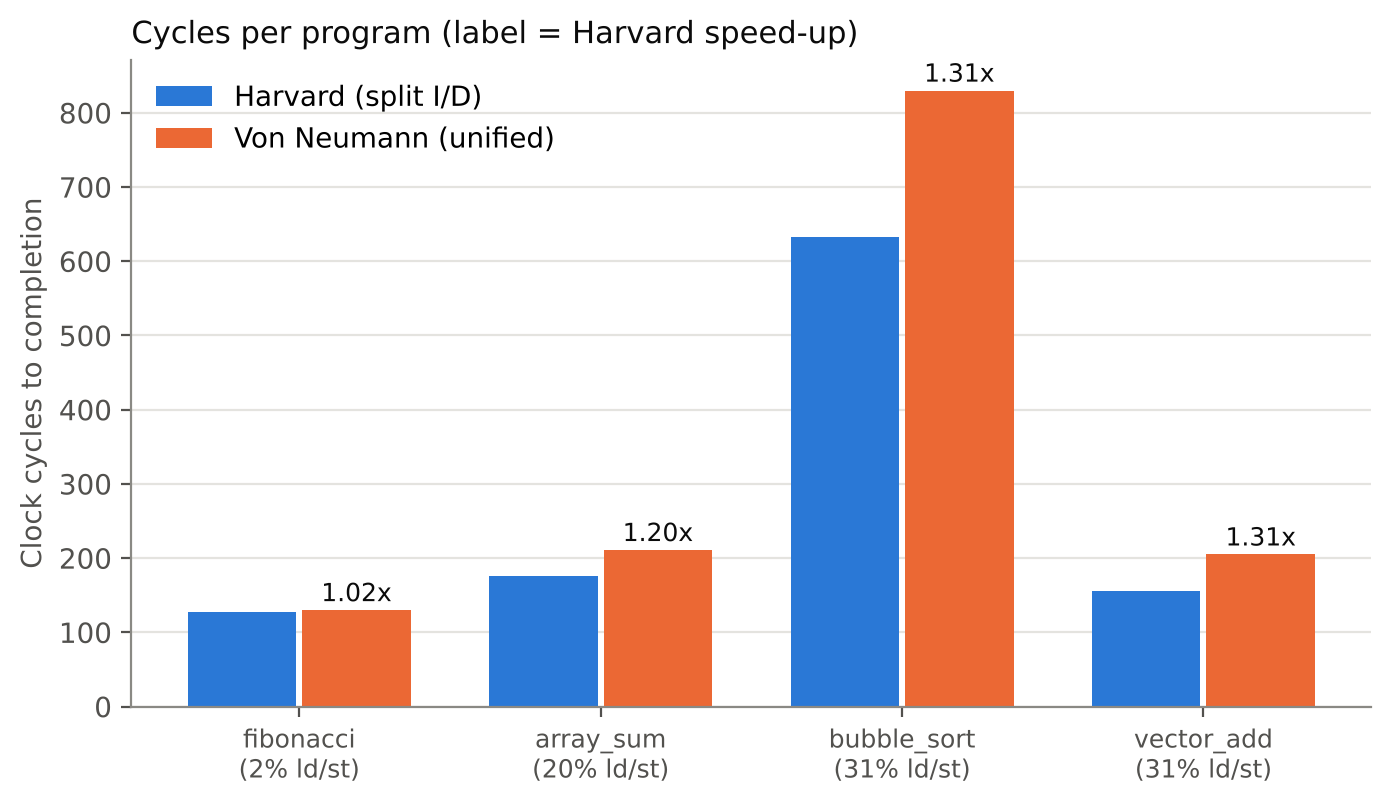
\includegraphics[width=\columnwidth]{cycles_comparison.png}
\caption{Cycles to completion for each program on both organisations.}
\label{fig:cycles}
\end{figure}

\subsection{Plan for Phase II}
Phase II will (i) add an optional shared lower-level memory behind small
instruction and data buffers to model a modified-Harvard hierarchy, (ii) add
multi-cycle main-memory latency so that average memory access time can be
reported, (iii) run synthesis to obtain resource utilisation and maximum
frequency, and (iv) extend the benchmark set and the comparison.

% ---------------------------------------------------------------------------
\section{Individual Contributions}
\begin{table}[h]
\caption{Contribution of each member (Phase I)}
\label{tab:contrib}
\centering
\renewcommand{\arraystretch}{1.15}
\begin{tabular}{p{0.24\columnwidth}p{0.68\columnwidth}}
\toprule
Member & Contribution \\
\midrule
Aaryan Yadav (2401010011) & Processor core: \texttt{pc.v}, \texttt{regfile.v}, \texttt{alu.v}, \texttt{imm\_gen.v}, \texttt{control\_unit.v} and their integration in \texttt{cpu\_core.v}; instruction-subset definition. \\
Shashwat Sinha (2401010438) & Instruction side and software: \texttt{imem.v}; Python assembler and golden-model ISS (\texttt{rv32\_asm.py}); the four test programs. \\
Shivam Mishra (2401010442) & Data side: \texttt{dmem.v}, \texttt{addr\_decoder.v}, \texttt{rw\_control.v}, \texttt{io\_regs.v}; address map; \texttt{harvard\_top.v} integration. \\
Himank Kaushik (2401010187) & Shared-memory baseline: \texttt{unified\_mem.v}, arbiter FSM in \texttt{vonneumann\_top.v}, \texttt{perf\_counters.v}; CPI model and comparison analysis. \\
Satyam Kumar (2401010429) & Verification and documentation: \texttt{tb\_top.v}, \texttt{tb\_addr\_decoder.v}, regression scripts, waveform figures, this report and the demo video. \\
\bottomrule
\end{tabular}
\end{table}

% ---------------------------------------------------------------------------
\begin{thebibliography}{00}
\bibitem{mca_projects} Rishihood University, ``Modern Computer Architecture: Projects 1--12, Architecture-oriented RTL projects,'' Course document, B.Tech (CS\&AI), 2026.
\bibitem{vonneumann1945} J. von Neumann, ``First draft of a report on the EDVAC,'' Moore School of Electrical Engineering, Univ. of Pennsylvania, 1945.
\bibitem{aiken1946} H. H. Aiken and G. M. Hopper, ``The automatic sequence controlled calculator,'' \textit{Electrical Engineering}, vol.~65, 1946.
\bibitem{backus1978} J. Backus, ``Can programming be liberated from the von Neumann style? A functional style and its algebra of programs,'' \textit{Commun. ACM}, vol.~21, no.~8, pp.~613--641, 1978.
\bibitem{wulf1995} W. A. Wulf and S. A. McKee, ``Hitting the memory wall: Implications of the obvious,'' \textit{ACM SIGARCH Comput. Archit. News}, vol.~23, no.~1, pp.~20--24, 1995.
\bibitem{smith1982} A. J. Smith, ``Cache memories,'' \textit{ACM Comput. Surv.}, vol.~14, no.~3, pp.~473--530, 1982.
\bibitem{patterson2020} D. A. Patterson and J. L. Hennessy, \textit{Computer Organization and Design RISC-V Edition: The Hardware/Software Interface}, 2nd~ed. Cambridge, MA, USA: Morgan Kaufmann, 2020.
\bibitem{hennessy2017} J. L. Hennessy and D. A. Patterson, \textit{Computer Architecture: A Quantitative Approach}, 6th~ed. Cambridge, MA, USA: Morgan Kaufmann, 2017.
\bibitem{harris2021} S. L. Harris and D. M. Harris, \textit{Digital Design and Computer Architecture: RISC-V Edition}. Morgan Kaufmann, 2021.
\bibitem{riscv_isa} A. Waterman and K. Asanovi\'{c}, Eds., \textit{The RISC-V Instruction Set Manual, Volume I: Unprivileged ISA}, Document Version 20191213, RISC-V Foundation, 2019.
\bibitem{arm_m3} ARM Ltd., \textit{Cortex-M3 Technical Reference Manual}, ARM DDI 0337, 2010.
\bibitem{picorv32} C. Wolf, ``PicoRV32 -- A size-optimized RISC-V CPU,'' GitHub repository. [Online]. Available: \url{https://github.com/YosysHQ/picorv32}
\bibitem{icarus} S. Williams, ``Icarus Verilog.'' [Online]. Available: \url{https://steveicarus.github.io/iverilog/}
\end{thebibliography}

\end{document}
